\newpage
\section{
\textbf{ {\Large 
بخش دوم: DHCP
}}}
\subsection{مقدمه}
همان‌طور که در درس خواندید، در یک شبکه‌ی لایه سوم، نیاز داریم تا اجزاء شبکه با ساختارهایی مانند IP با هم ارتباط برقرار کنند\footnote
{وب‌گاه
\lr{\url{https://en.wikibooks.org/wiki/Communication\_Networks/DHCP\_Protocol}}
مرجع توضیحات مقدمه و تصاویر مربوط به پروتکل DHCP است.
}. از این رو باید به هر گره در این شبکه یک IP نسبت دهیم. انتساب IP روش‌های مختلفی دارد که سه روش کلی آن به صورت زیر است:
\begin{itemize}
\item
دستی: در این روش، مدیر شبکه به صورت دستی به هر عضو شبکه یک IP نسبت می‌دهد. این روش کمی سخت است و زمان بیشتری نسبت به سایر روش‌های دیگر نیاز دارد، اما در عوض امن ترین روش برای اختصاص IP است.

\item
خودکار: در این روش به صورت خودکار به هر گره شبکه یک IP جدید اختصاص داده می‌شود.

\item
پویا: در این روش در واقع برای هر درخواستی از جانب اعضای شبکه، یک قرارداد وضع می‌شود و IP جدیدی براساسِ  این قرارداد به آن گره اختصاص پیدا می‌کند. در نتیجه اعضا می‌توانند به شبکه وارد یا از آن خارج شوند.
\end{itemize}

روش پویا در این میان، پرکاربردترین روش برای اختصاص IP است و تمرکز تمرین نیز روی این بخش است.

\subsection{مقدمه‌ای بر \lr{DHCP}}

پروتکل 
\lr{Dynamic Host Configuration Protocol (DHCP)}
در واقع به نوعی نسخه‌ی به‌روز‌ شده‌ی پروتکل 
\lr{Bootstrap Protocl (BOOTP)}
است و به صورت عقبگرد از این پروتکل پشتیبانی می‌کند.

همان‌طور که گفته شد، این پروتکل مواقعی کاربرد دارد که اعضای شبکه به صورت موقتی به شبکه وارد و از آن خارج می‌شوند. در این مواقع، ما نیاز به دست‌کم یک کارگزار DHCP داریم. وظیفه کارگزار DHCP این است که به عنوان مدیر شبکه عمل کند و آی‌پی‌ها را مدیریت کند.

  هر عضو شبکه که درخواستی دارد، به این کارگزار درخواست ارسال می‌کند و او به ازای مک آدرسی که درخواست را ارسال کرده،  یک آی‌پی پیشنهاد می‌دهد. ممکن است در شبکه چند کارگزار DHCP وجود داشته باشند در نتیجه چند پیشنهاد برای این کارخواه می‌آید. او یکی از آن‌ها را انتخاب می‌کند و پیام را به کارگزار مربوطه می‌فرستد. کارگزار در صورت موافقت، پیامی را به همگان broadcast می‌کند تا سایر پیشنهادات را لغو کند و کارخواه \LTRfootnote{client} این IP را بگیرد.

بسته به نوع پیکربندی شبکه، ممکن است در شبکه لایه دو، کارگزار موجود باشد یا کارگزار در یک شبکه دیگر باشد. در ادامه یک مثلا از فرآیند‌های DHCP برای شما آمده است.

\begin{enumerate}
\item
 فرض کنید یک عضو جدید به شبکه اضافه شده است و می‌خواهد آی‌پی دریافت کند. پس ابتدا پیامی مبنی بر DHCPDISCOVER در کل شبکه broacast می‌کند. هدف از این بسته پیدا کردن کارگزاران DHCP است. محتوای این بسته به این‌صورت است که مک آدرس مبدأ را شامل می‌شود و از درگاه ۶۸ به آی‌پی
 \lr{255.255.255.255}
 و درگاه 
 ۶۷
 ارسال می‌شود. همچنین درخواست می‌تواند شامل آی‌پی درخواستی و مدت زمان اعتبار این آی‌پی باشد.
 
 \item
 حال این بسته به دست \lr{DHCP rely} می‌رسد و او  چون آدرس \lr{DHCP Server} را می‌داند بسته را برای \lr{DHCP Server} به صورت unicast ارسال می‌کند. همچنین فیلد giaddr را با آدرس gateway 
 \lr{10.1.2.9}
 پر می‌کند تا کارگزار DHCP بداند که برای کدام زیرشبکه \LTRfootnote{sub-network} باید آی‌پی اختصاص دهد.  
 \begin{figure}[h!]
	\begin{center}
 		\caption{ارسال DHCPDISCOVER از طرف گره‌ی جدید }
		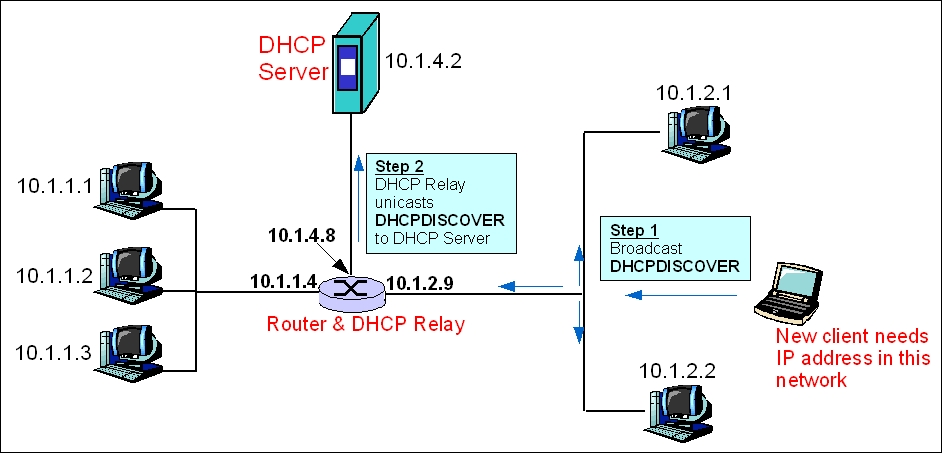
\includegraphics[scale=.4]{DHCP1.jpg}
	\end{center}
\end{figure}

 \item
 حال که بسته دست کارگزار رسید، یک آی‌پی جدید پیشنهاد می‌دهد و بسته حاوی آدرس جدید یعنی بسته‌ی DHCPOFFER را  broadcast می‌کند.
 
 \item
 سپس 
 \lr{DHCP Relay}
  بسته‌ی DHCPOFFER را تنها روی واسط مورد نظر broacast می‌کند.
 
 \item
 حال کارخواه و سایر اعضای شبکه بسته پیشنهادی را می‌بینند و کارخواه ما در صورت تمایل، آی‌پی پیشنهادی را قبول می‌کند.

 \begin{figure}[h!]
	\begin{center}
 		\caption{ارسال بسته‌ی DHCPOFFER}
		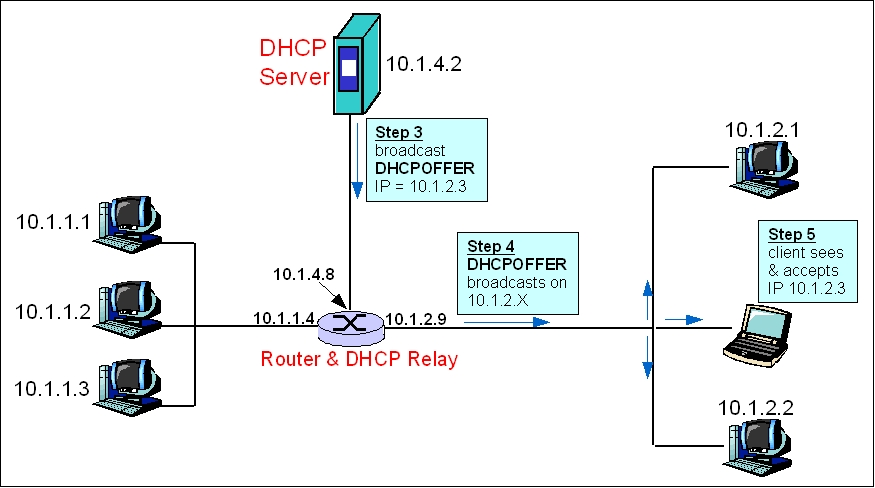
\includegraphics[scale=.4]{DHCP2.jpg}
	\end{center}
\end{figure}

 \item
 کارخواه، در صورت قبول پیشنهاد، بسته DHCPREQUEST را برای کارگزار می‌فرستد.
  
 \item
\lr{DHCP rely} بسته را به سرور می‌فرستد.

\item
سرور بسته DHCPACK را در صورت تایید برای تمام اعضای شبکه broadcast می‌کند تا سایر DHCPOFFER ها از بین بروند و این کارخواه تنها همین آی‌پی را بگیرد. در صورتی که موافق نباشد می‌تواند بسته DHCPNACK را بفرستد و پس از این کارخواه چاره‌ای ندارد جز اینکه همه مراحل را از 
اول شروع کند. 
 \begin{figure}[h!]
	\begin{center}
 		\caption{ارسال بسته‌ی DHCPREQUEST و دریافت پاسخ}
		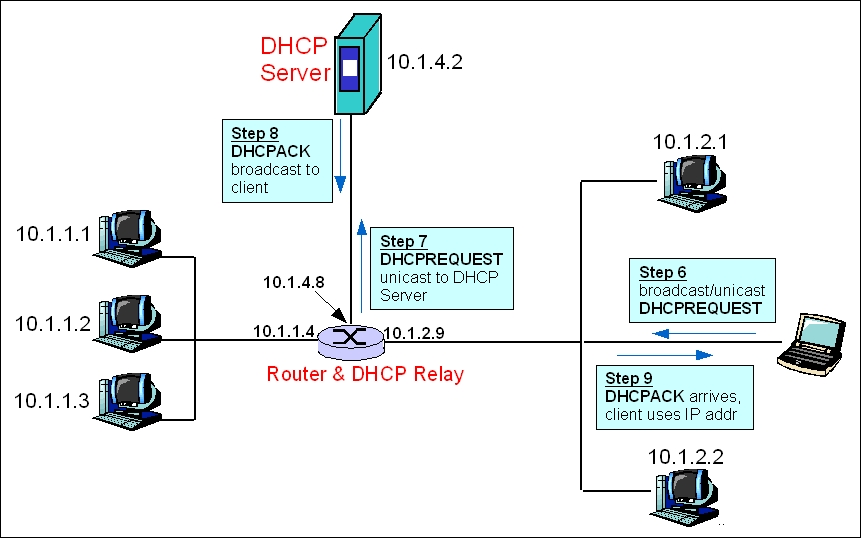
\includegraphics[scale=.4]{DHCP3.jpg}
	\end{center}
\end{figure}
\end{enumerate}

به‌جز بسته‌های مطرح‌شده در سناریو بالا، بسته‌های دیگری نیز می‌توانند در این پروتکل وجود داشته باشند مانند درخواست تجدید زمان، درخواست رهاسازی آی‌پی گرفته شده، درخواست دریافت اطلاعات بیشتر.

از نظر امنیتی، این پروتکل ناامن است، چرا که روش درستی برای احراز هویت در آن وجود ندارد. برای مثال کارگزار نمی‌داند آیا مک آدرسی که درخواست آی‌پی جدید دارد واقعاً در شبکه موجود است یا یکی از گره‌ها این درخواست را داده است. یا مثلا کارخواه نمی‌داند پیشنهادات از سوی یک کارگزار واقعی است یا خیر.